\documentclass[10pt,landscape]{article}

\usepackage[boxruled, linesnumbered]{algorithm2e}
\usepackage{multicol}
\usepackage{calc}
\usepackage{ifthen}
\usepackage[landscape]{geometry}
\usepackage{graphicx}
\usepackage{amsmath, amssymb, amsthm}
\usepackage{latexsym, marvosym}
\usepackage{pifont}
\usepackage{lscape}
\usepackage{graphicx}
\usepackage{array}
\usepackage{booktabs}
\usepackage[bottom]{footmisc}
\usepackage{tikz}
\usetikzlibrary{shapes}
\usepackage{pdfpages}
\usepackage{wrapfig}
\usepackage{enumitem}
\setlist[description]{leftmargin=0pt}
\usepackage{xfrac}
\usepackage[pdftex,
            pdfauthor={Daniel Fernandez},
            pdftitle={ML CheatSheet},
            pdfsubject={A cheatsheet pdf and reference guide for Statistics and ML concepts (from linear regression to DNN).},
            pdfkeywords={machineLearning} {statistics} {cheatsheet} {pdf} {cheat} {sheet} {regression} {equations}
            ]{hyperref}
\usepackage[
            open,
            openlevel=2
            ]{bookmark}
\usepackage{relsize}
\usepackage{rotating}

 \newcommand\independent{\protect\mathpalette{\protect\independenT}{\perp}}
    \def\independenT#1#2{\mathrel{\setbox0\hbox{$#1#2$}%
    \copy0\kern-\wd0\mkern4mu\box0}}

\newcommand{\noin}{\noindent}
\newcommand{\logit}{\textrm{logit}}
\newcommand{\var}{\textrm{Var}}
\newcommand{\cov}{\textrm{Cov}}
\newcommand{\corr}{\textrm{Corr}}
\newcommand{\N}{\mathcal{N}}
\newcommand{\Bern}{\textrm{Bern}}
\newcommand{\Bin}{\textrm{Bin}}
\newcommand{\Beta}{\textrm{Beta}}
\newcommand{\Gam}{\textrm{Gamma}}
\newcommand{\Expo}{\textrm{Expo}}
\newcommand{\Pois}{\textrm{Pois}}
\newcommand{\Unif}{\textrm{Unif}}
\newcommand{\Geom}{\textrm{Geom}}
\newcommand{\NBin}{\textrm{NBin}}
\newcommand{\Hypergeometric}{\textrm{HGeom}}
\newcommand{\HGeom}{\textrm{HGeom}}
\newcommand{\Mult}{\textrm{Mult}}

\geometry{top=.4in,left=.2in,right=.2in,bottom=.4in}

\pagestyle{empty}
\makeatletter
\renewcommand{\section}{\@startsection{section}{1}{0mm}%
                                {-1ex plus -.5ex minus -.2ex}%
                                {0.5ex plus .2ex}%x
                                {\normalfont\large\bfseries}}
\renewcommand{\subsection}{\@startsection{subsection}{2}{0mm}%
                                {-1explus -.5ex minus -.2ex}%
                                {0.5ex plus .2ex}%
                                {\normalfont\normalsize\bfseries}}
\renewcommand{\subsubsection}{\@startsection{subsubsection}{3}{0mm}%
                                {-1ex plus -.5ex minus -.2ex}%
                                {1ex plus .2ex}%
                                {\normalfont\small\bfseries}}
\makeatother

\setcounter{secnumdepth}{0}

\setlength{\parindent}{0pt}
\setlength{\parskip}{0pt plus 0.5ex}

% -----------------------------------------------------------------------

\usepackage{titlesec}

\titleformat{\section}
{\color{blue}\normalfont\large\bfseries}
{\color{blue}\thesection}{1em}{}
\titleformat{\subsection}
{\color{cyan}\normalfont\normalsize\bfseries}
{\color{cyan}\thesection}{1em}{}
% Comment out the above 5 lines for black and white

\begin{document}

\raggedright
\footnotesize
\begin{multicols*}{3}

% multicol parameters
% These lengths are set only within the two main columns
%\setlength{\columnseprule}{0.25pt}
\setlength{\premulticols}{1pt}
\setlength{\postmulticols}{1pt}
\setlength{\multicolsep}{1pt}
\setlength{\columnsep}{2pt}

%%%%%%%%%%%%%%%%%%%%%%%%%%%%%%%%%%%%
%%% TITLE
%%%%%%%%%%%%%%%%%%%%%%%%%%%%%%%%%%%%

\begin{center}
    {\color{blue} \Large{\textbf{ML/Stats Cheatsheet}}} \\
   % {\Large{\textbf{Probability Cheatsheet}}} \\
    % comment out line with \color{blue} and uncomment above line for b&w
\end{center}

%%%%%%%%%%%%%%%%%%%%%%%%%%%%%%%%%%%%
%%% ATTRIBUTIONS
%%%%%%%%%%%%%%%%%%%%%%%%%%%%%%%%%%%%

\scriptsize

Compiled by Daniel Fernandez (used template from http://wzchen.com and Joe Blitzstein).

\begin{center}
    Last Updated \today
\end{center}

% Cheatsheet format from
% http://www.stdout.org/$\sim$winston/latex/

%%%%%%%%%%%%%%%%%%%%%%%%%%%%%%%%%%%%
%%% BEGIN CHEATSHEET
%%%%%%%%%%%%%%%%%%%%%%%%%%%%%%%%%%%%


\section{Machine Learning Definitions}\smallskip \hrule height 2pt \smallskip

    \subsection{Supervised and Unsupervised Learning}

    \begin{minipage}{\linewidth}
        \centering
        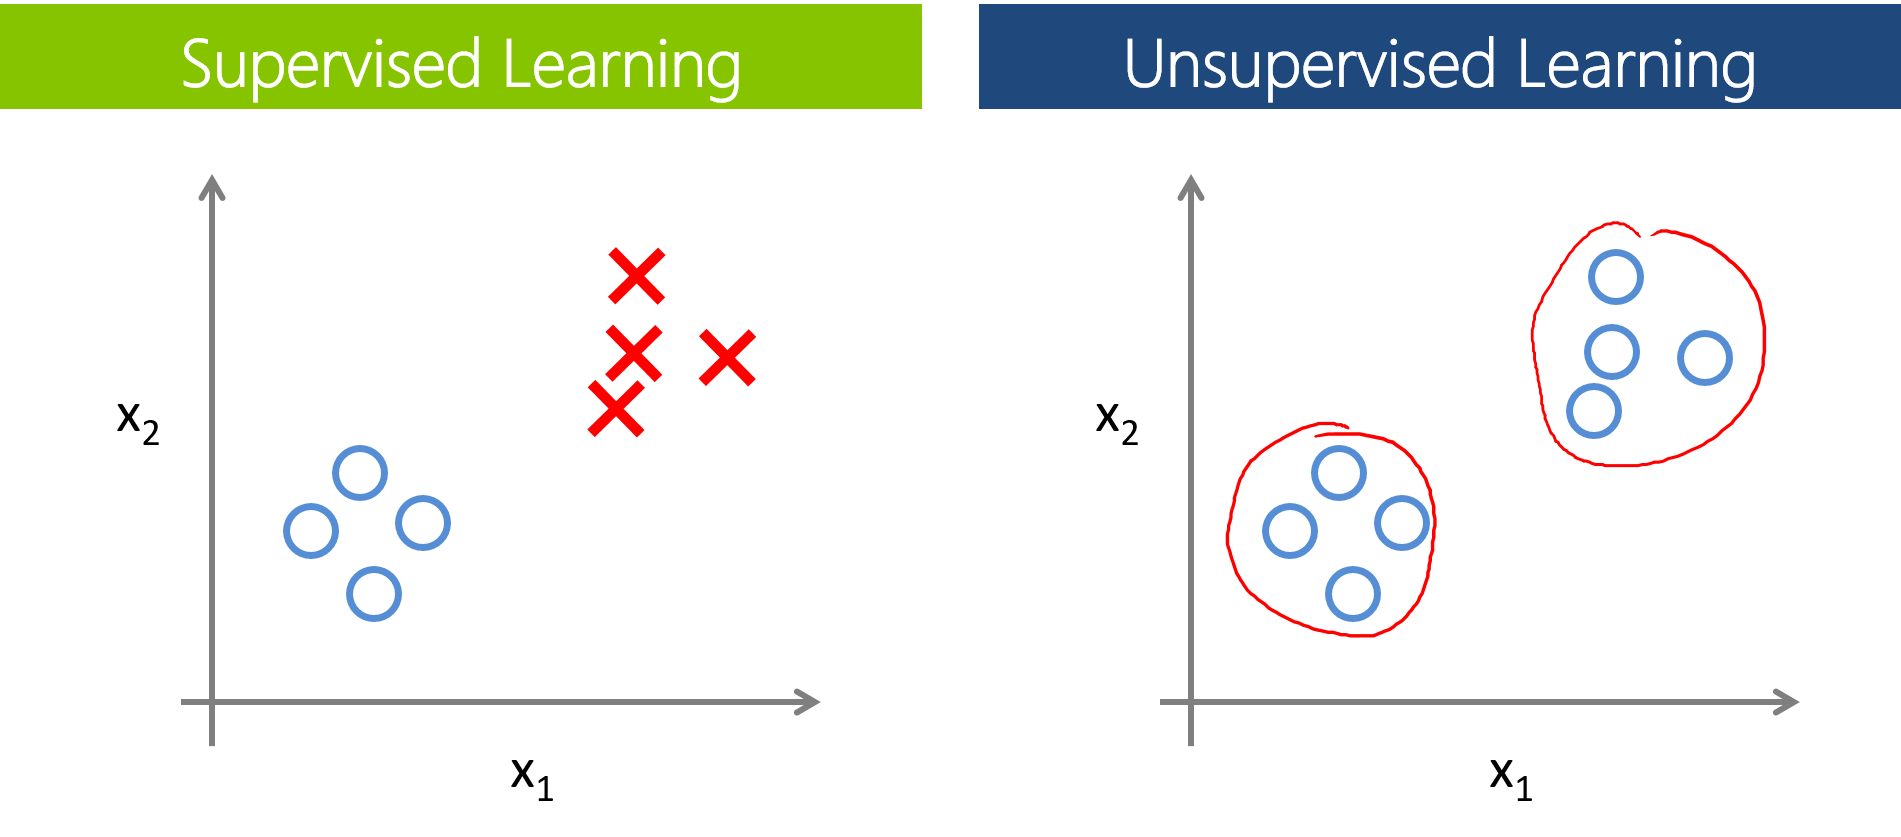
\includegraphics[width=2in]{figures/supervised_unsupervised.png}
    \end{minipage}

    Let us first define our response as a vector of dimension n, $Y_n$; and
    our predictors/features/variables as a matrix of dimension $n \times p$,
    $X_{n\times p}$ (i.e., $p$ predictors).

    In Supervised Learning one aim to train a model to classify/predict
    a categorical/numerical output $Y$, using features/variables $X$.

    In Unsupervised Learning one aims to find patterns/summaries/groups
    in the given data - common tasks are clustering,
    and dimensionality reduction.

    \begin{minipage}{\linewidth}
            \centering
            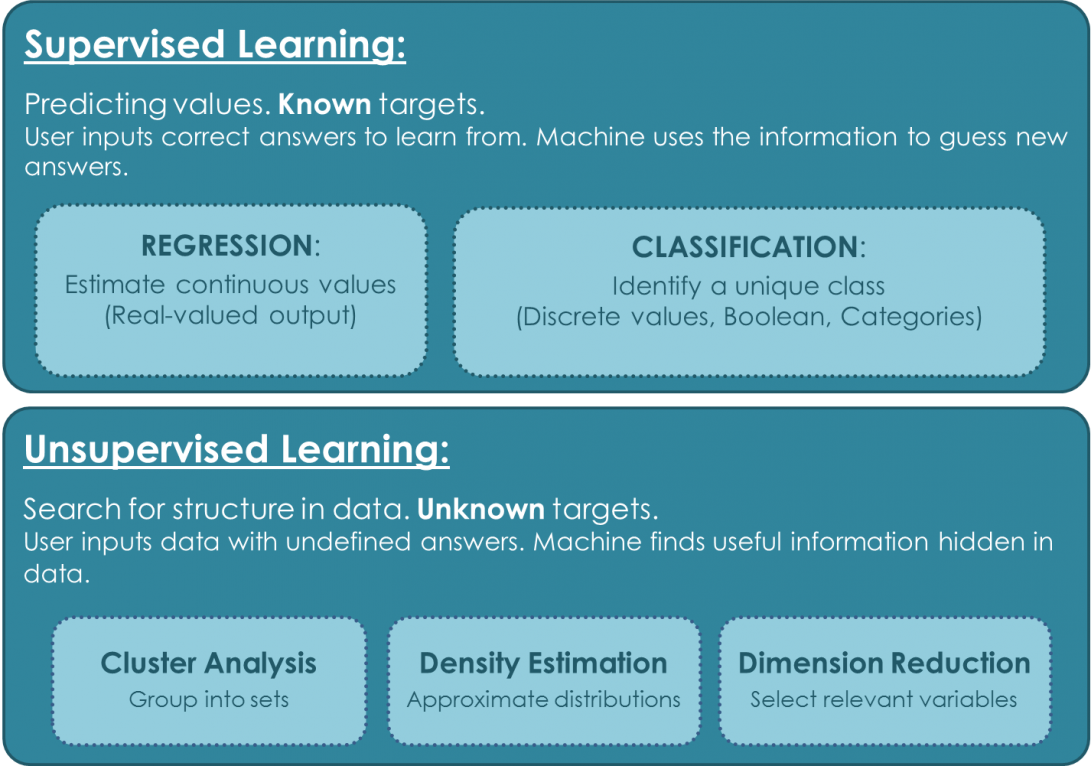
\includegraphics[width=2in]{figures/learn_methods_summary.png}
    \end{minipage}

    \subsection{Fundamental Ideas}

    \begin{description}
        % \item[Disjoint Events] - ${\bf A}$ and ${\bf B}$ are disjoint when they cannot happen simultaneously, or
        %   \begin{align*}
        %     P({\bf A} \cap {\bf B}) &= 0\\
        %     {\bf A} \cap {\bf B} &= \emptyset
        %   \end{align*}
        \item[Curse of Dimensionality] as the number of features grows one need exponentially more
        data points to provide local generalizations (i.e., KNN).

        \item[Bias and Variance Tradeoff]  The mean squared error (loss) of my model, $\hat{y}$ fit to the real data, $y$,
        exhibits a tradeoff between overparametrized models (e.g., splines) exhibiting low-bias, high-variance; and
        underparametrized models exhibiting high bias, low variance.  Mathematically,
               \begin{align*}
                E\left[ \left( \hat{y}-y \right)^2 \right] = \var(\hat{y}) + [Bias(\hat{y})]^2
               \end{align*}
        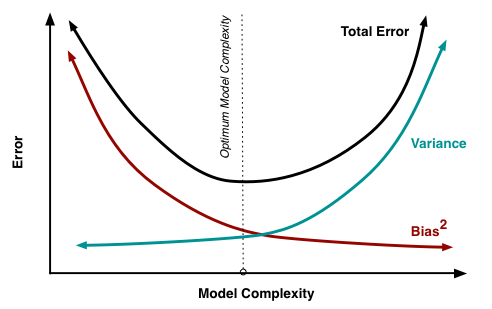
\includegraphics[width=2in]{figures/biasvariance.png}
        \item[Train, validation and test]  In order to prevent overfitting, and having better measures of the model performance OOS
        one technique is to divide the set of data $(X,Y)$ into train, validate, test.  The train-validate set can be done using
        K-fold cross validation, or rolling cross-validation (in case of time series) along with hyper-parameter optimization
        (grid, bayesian or random search).  One can optimize the model hyperparameters using
        The test set ensures that we have an unbias and objective measure of the error after the model
        hyperparameters have been optimized.

        \item[Large $p$, small $n$ Problem].  When $p >> n$ it is commonly
        called an large $p$, small $n$ problem. I.e., a large feature space for a relatively small
        number of observations.  Methods to tackle this problem rely on variable selection, and
        dimension reduction techniques.  Examples easily arise in statistical genetics
        (large number of genes/SNPs ($~20k$/$600k$ in humans),
        small number of observations of people with a given disease.

        \item[Admisibility]. An admissible decision rule is a rule for making a decision
        such that there is not any other rule that is always "better"
        (as defined by MSE for example) than it.

    \end{description}

    \subsection{Performance Metrics}

    \begin{description}

    \item[continuous response]

    \item[Mean Squared Error (MSE)] $E\left[(y-\hat{y})^2 \right]$.  \\
    It weights larger differences (outliers) more heavily
    (squares are larger as the error gets larger). \\
    The mean of $Y$ (when no $X$) minimizes the MSE. \\

    \item[Mean Absolute Error (MAE)]. $E\left|y-\hat{y}\right|$. \\
    It is less sensitive to large differences. \\
    The median of $Y$ minimizes the MAE. \\

    \begin{minipage}{\linewidth}
        \centering
        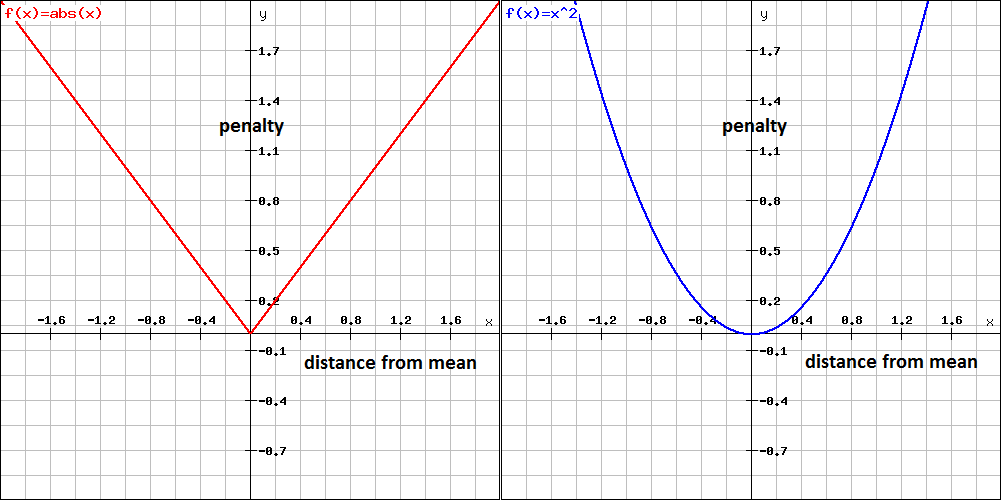
\includegraphics[width=3in]{figures/mse1.png}
    \end{minipage}

    \begin{minipage}{\linewidth}
        \centering
        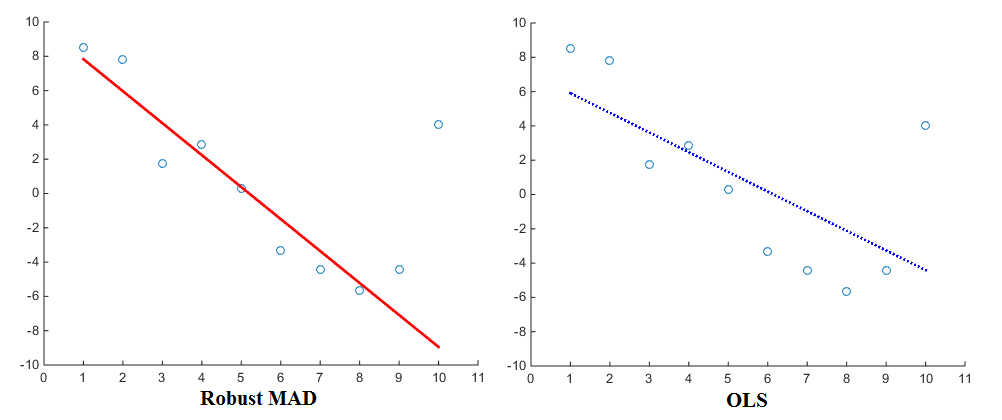
\includegraphics[width=3in]{figures/mse2.png}
    \end{minipage}

    Other measures are the Mean Absolute percentage error (MAPE),
    or the mean squared percentage error (MSPE). \\

    When taking the median the sensitivity to outliers is further reduced,
    but it comes with an intuitive caveat. Remember that the median of the
    values 1, 2 and 3, and the median the values 1, 2 and 999, are both 2.
    If the numbers in the two series above were the amount of money you would
    risk to lose as a consequence of participating in two different investment
    alternatives over the next day, evaluating the risk of these two investments
    by median loss would clearly be irrational.


    \item[categorical response]

    \item[binary response]

    \end{description}

    \subsection{Information Theory}

    \begin{description}

    \item[Information Content] The information content is related to the
    number of binary decisions required to find the information.  I.e., Is it head or tail?
    $\log_2(2) = 1$.  Which nucleotide? $\log_2(4) = 2$. \\
    Generally, for a discrete random variable taking value $i$, $I(p_i) = -\log_2(p_i)$. \\

    \textbf{properties}. \\
    (1) $I(p)$ is anti-monotonic \\
    (2) $I(0)$ is undefined, \\
    (3) $I(p) \geq 0$ - information is a non-negative quantity \\
    (4) $I(1) = 0$ - events that always occur contain no information \\
    (5) $I(p_1 \times p_2) = I(p_1) + I(p_2)$ - information due to indenpendent
    events is additive.

    \item[Entropy] Entropy quantifies the amount of uncertainty
    inherent in the value of a random variable (or the outcome of
    a random process).  Specifically, it is the average information
    of all possible outcomes of the random variable.

    \begin{align*}
    H(X) = E[I(X)] = E[-\log p(x)] = -\sum_{i=1}^{n} p(x_i) \log_2 p(x_i)
    \end{align*}

    \item[Joint Entropy] The entropy of the pairing $(X,Y)$.  If  they are independent
     then it is the sum of $H(X)+H(Y)$.

     \begin{align*}
         H(X,Y) = E[I(X,Y)] = E_{X,Y}[-\log p(x,y)] = -\sum_{x,y} p(x,y) \log_2 p(x,y)
     \end{align*}

    \item[Conditional Entropy] Or, conditional uncertainty of $Y$ given $X$.

     \begin{align*}
         H(Y|X) &=& E_X[H(Y|x)] = -\sum_{x} p(x) H(Y|x) \\
                &=& -\sum_{x} p(x) \sum_{y} p(y|x) \log p(y|x) \\
                &=& -\sum_{x,y} p(x,y) \log \frac{p(x,y)}{p(x)}
     \end{align*}

     \begin{align*}
        H(Y|X) = H(X,Y) - H(X)
     \end{align*}

    \item[Mutual Information] It measures the amount of information that can be obtained about one random variable by
    observing another random variable.

     \begin{align*}
         I(X,Y) = H(Y) - H(Y|X)
     \end{align*}

     It is symmetric in $X$ and $Y$,

     \begin{align*}
        I(X,Y) = I(Y,X) = H(X) + H(Y) - H(X,Y)
     \end{align*}

     It can be expressed as the average KL (information gain) between the posterior probability of $X$ given the
     value of $Y$, and the prior distribution on $X$.

     \begin{align*}
             I(X,Y) = E_{p(y)}[D_{KL}(p(X|Y=y)||p(X))] = D_{KL}(p(X,Y)||p(X)p(Y))
     \end{align*}


    Graphically,

    \begin{minipage}{\linewidth}
        \centering
        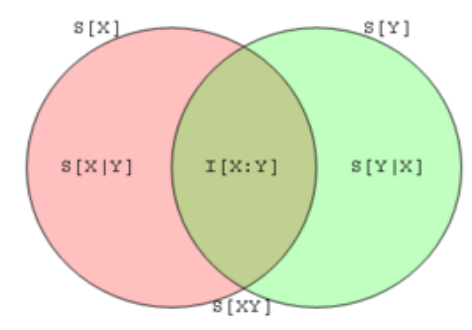
\includegraphics[width=2in]{figures/informationTheory.png}
    \end{minipage}

    \item[Kullback-Leibler divergence,] \textbf{or information gain, or relative entropy}. \\
    I must transmit $Y$. How many bits
    on average would it save me if both ends of the line knew $X$?.  \\
    It is also interpreted as the difference between two probability distributions $P$ and $Q$.  \
    It is not symmetric in $P$ and $Q$.  In applications, $P$ typically
    represents the "true" distribution of data, observations, or a precisely calculated theoretical distribution,
    while $Q$ typically represents a theory, model, description, or approximation of $P$. \\
    The Kullback–Leibler divergence is sometimes also called the information gain achieved if
    $P$ is used instead of $Q$. In Bayesian statistics the Kullback–Leibler divergence can be used as a
    measure of the information gain in moving from a prior distribution to a posterior distribution. \\
    It is also called the relative entropy of $P$ with respect to $Q$.

    \begin{align*}
        D_{KL}(p(X)||q(X)) &=& \sum_x -p(x)\log q(x) - \sum_x -p(x)\log p(x) \\
                           &=& \sum_x p(x) \log \frac{p(x)}{q(x)}
    \end{align*}

    \begin{minipage}{\linewidth}
        \centering
        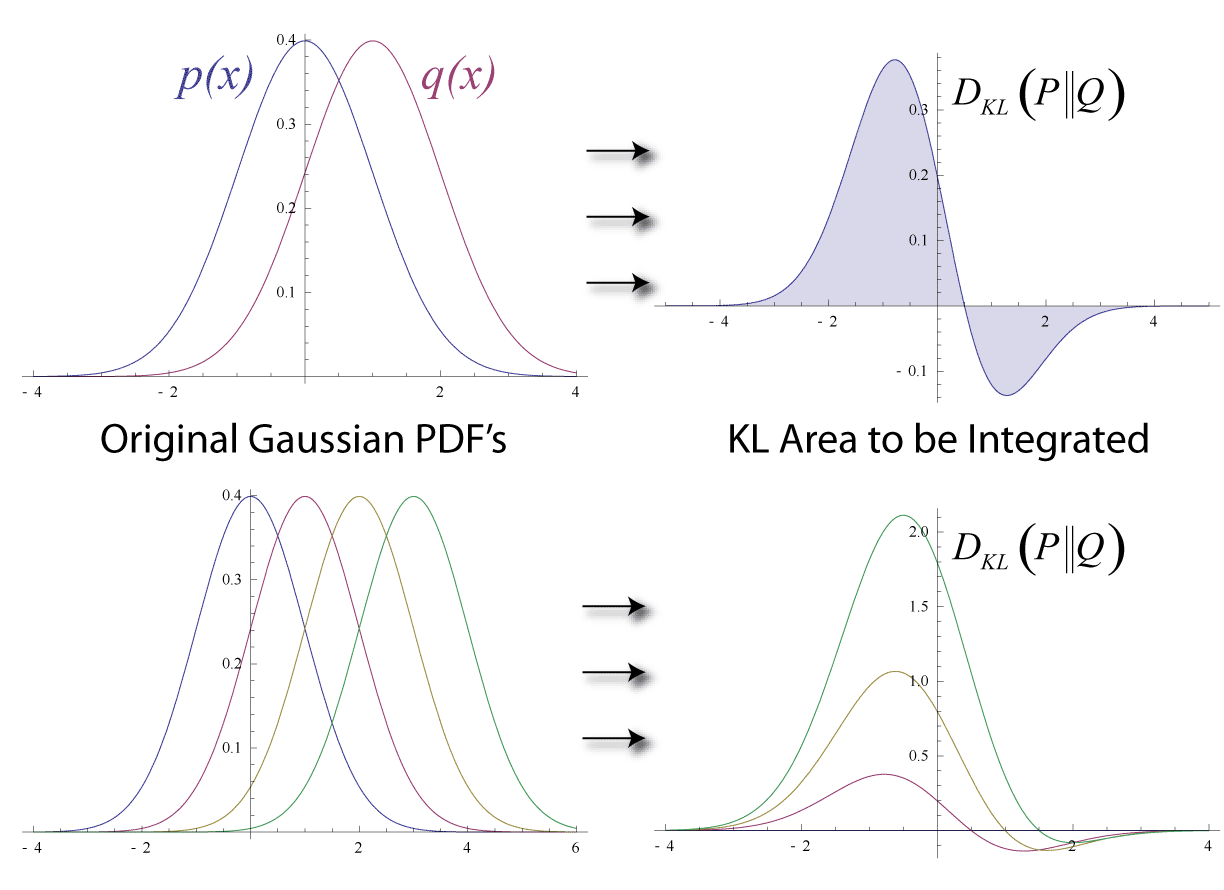
\includegraphics[width=2.5in]{figures/kl.png}
    \end{minipage}

    The assymetry is clear from the picture.  We integrate w/r to p(x)

    \end{description}

\section{Linear Regression}



\section{Decision Trees}

    Tree-based methods partition the feature space into a set of rectangles
    and then fit a simple model in each one.  \\

    For binary $X$ and binary $Y$, one would have $n-$OR, any, (linear complexity),
    and $n-$XOR, odd parity, ($2^p$ exponential complexity).  Thus, the space of all
    possible deicsion trees is extremely large, encompassing $2^{2^n}$ possible trees
    (double exponential, very fast grow).

    \begin{minipage}{\linewidth}
        \centering
        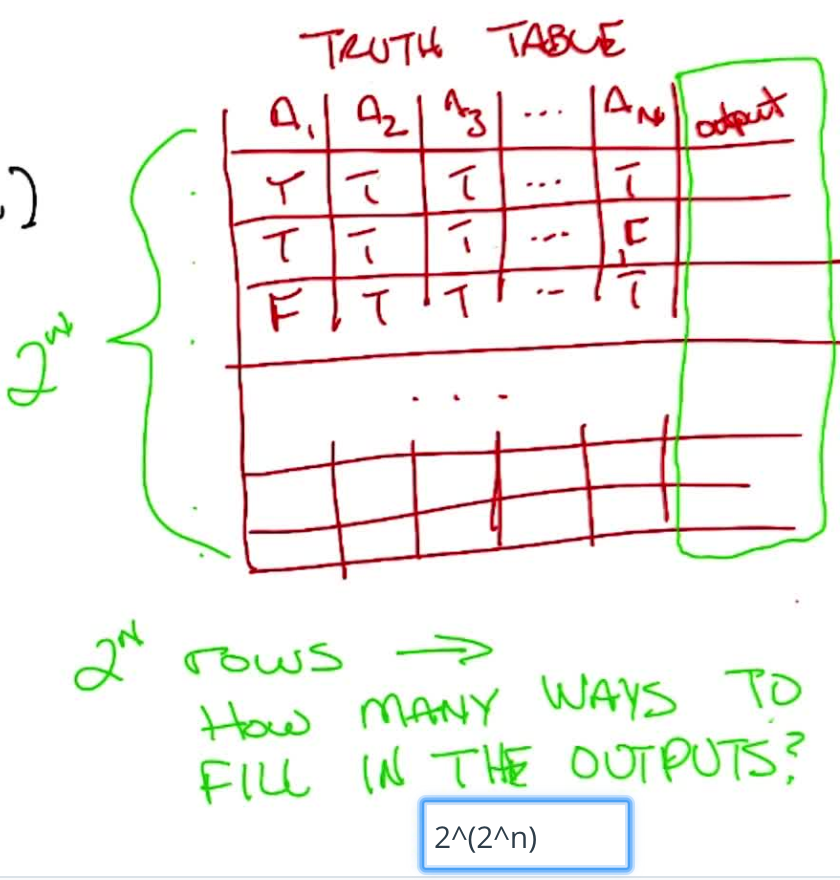
\includegraphics[width=2in]{figures/dtcomplexity.png}
    \end{minipage}

    One cannot guarantee to find the optimal tree, best one can do is to use greedy-search methods.
    The most popular methods are CART and $ID3 \rightarrow C4.5 \rightarrow C5.0$.

%    \begin{algorithm}[H]
%            \SetAlgoLined
%            Take all the data $Y$ \\
%            Consider all possible values of all variables in $X=(X_1,\ldots,X_p)$ \\
%            Select the variable/value $(X_j=t_1)$ that produces the greatest
%            separation of values in target $Y$ -- $(X_j=t_1)$ is called a Split. \\
%            \uIf{$ X_j < t_1$}{
%                Send data $Y$ to the left\;
%              }
%            \Else{
%                Send data $Y$ to the right \;
%            }
%            Repeat same process on these left and right nodes.
%        \caption{Recursive Partioning Idea}\label{alg:decisionTreeAlgo}
%    \end{algorithm}

    \begin{algorithm}[H]
        \SetAlgoLined
        \While{examples not perfectly classified} {
        Pick $X_j$ that "best" separates $Y$ \\
        Assign $X_j$ as decision feature for node \\
        For each value of $X_j$ create a descendant of node \\
        Assign training examples $Y$ to each leaf descendant of node
        }
    \caption{ID3 Top Down Learning Algorithm}\label{alg:id3algo}
    \end{algorithm}

    \begin{description}

    \item[Maximum Gain]  It is defined as the gain in separation
    by adding a new node $X_j$ to the decision tree. \\

    Common measures are the gini index, and the information gain. \\

    The information gain is defined as,

    \begin{align*}
        IG = H(parent) - [weighted_average]H(children)
    \end{align*}

    This measure has a major selection bias for $X_j$ categorical that takes multiple values.

    \item[Stop criterion and overfitting] Check accuracy in the cross validation set
    before decide to expand the tree.  Alternatively, do the full tree, and then
    do prunning.

    \item[Overall Considerations]
    Decision trees exhibit restriction bias, i.e., one only consider
    functional forms in the form of a tree.  \\
    They also exhibit a preference/inductive bias (certain trees
    are prefered more than others):  Trees with good splits at the top,
    prefers ones that give better classification accuracy. \\
    For continuous features, one can take ranges, and use them more than one time in the tree. \\
    For regression (instead of classification) the split criteria based on MSE, and the output
    could be a local linear fit.

    \begin{minipage}{\linewidth}
        \centering
        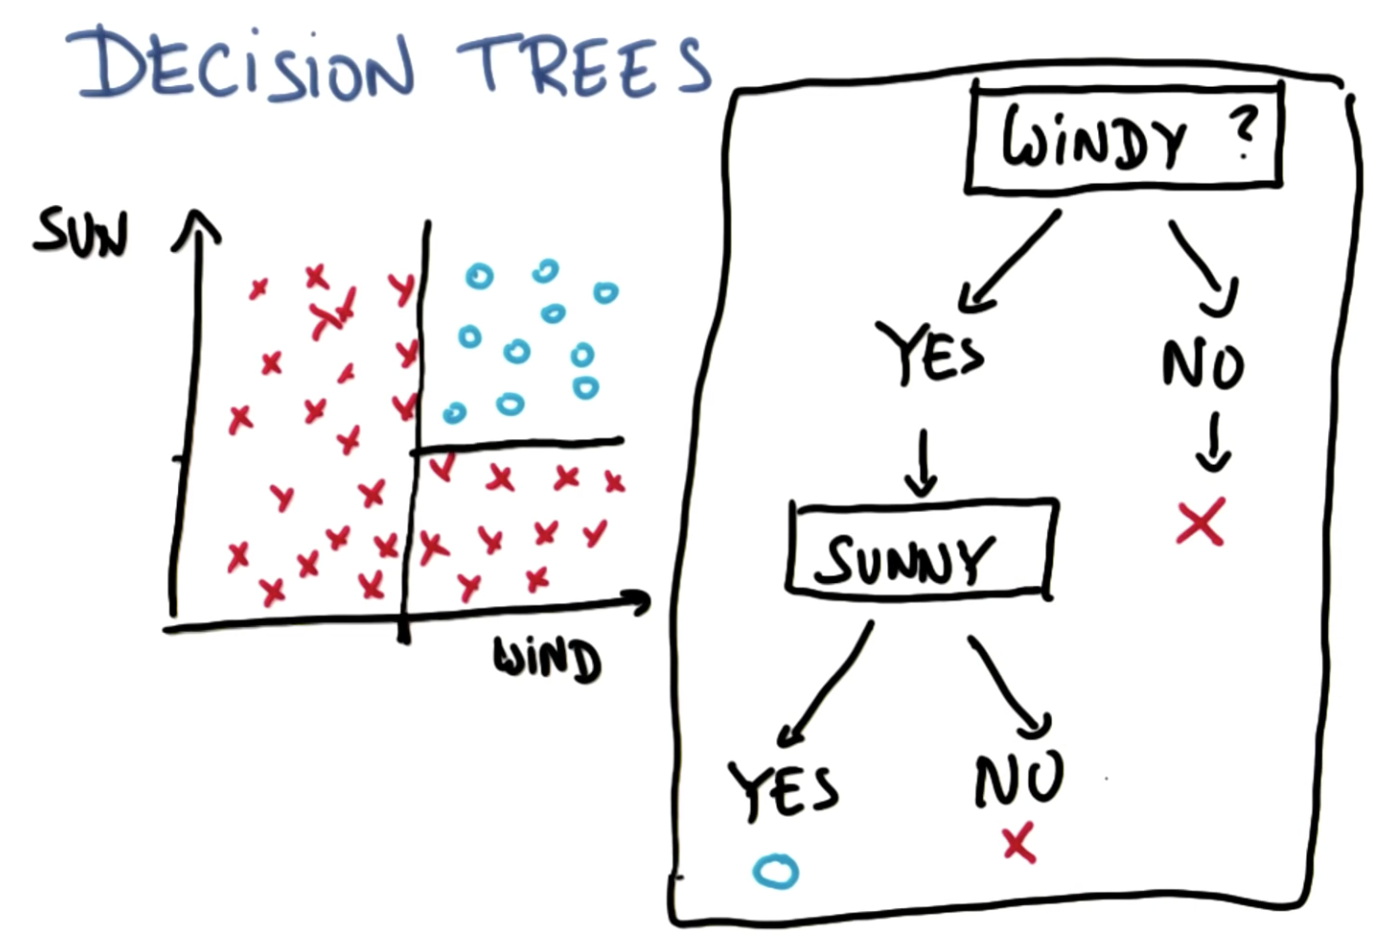
\includegraphics[width=2in]{figures/dtexample.png}
    \end{minipage}

    \end{description}

\section{Neural Networks}



\end{multicols*}

\end{document}
